\documentclass{lecture}

%\setbeameroption{show notes on second screen}
\usepackage{listliketab}
\usepackage{url}
\usepackage{xspace}
\usepackage{graphicx}
\usepackage{LI}
\usepackage{etex}
\usepackage{booktabs}
\usepackage{color}
\usepackage{latexsym}
\usepackage{tipa}
%\usepackage{wasysym}
\usepackage{tipa}
\usepackage{tikz}
\usepackage{tikz-qtree}
%\usepackage{textpos}
%\usepackage{MnSymbol}
\usetikzlibrary{arrows,automata,calc,positioning,through}
%\usepackage{verbatim} % for comment blocks
%\usepackage{ulem} % for strikethrough (sout)
\usepackage{pifont}
%\usepackage{ucs}
\usepackage[utf8]{inputenc}
\usepackage[T1]{fontenc}
%\usepackage{pylistings}
\usepackage{amsmath}
\usepackage{multirow}


\usefonttheme{professionalfonts} % using non standard fonts for beamer
\usefonttheme{serif} % default family is serif
%\setmainfont{fourier}

\definecolor{darkgreen}{cmyk}{0.74,0.06,0.98,0.2}

\newcommand{\red}[1]{\textcolor{usydred}{#1}}
\newcommand{\green}[1]{\textcolor{darkgreen}{#1}}
\newcommand{\blue}[1]{\textcolor{usydblue}{#1}}
\newcommand{\gold}[1]{\textcolor{usydyellow}{#1}}

%\usepackage{beamerthemesplit}

%\usepackage{javalistings}
%\usepackage{cpplistings}
\beamertemplatenavigationsymbolsempty
%\setbeamertemplate{navigation symbols}{}
%\setbeamertemplate{bibliography item}[text]


\usepackage[style=authoryear]{biblatex}
\renewcommand*\bibopenparen{[}
\renewcommand*\bibcloseparen{]}
\addbibresource{slides.bib}

\title{A Practical Algorithm for Topic Modling with Provable Guarantees}
\author[Vanush \& Kristy]{Sanjeev Arora\\
		Rong Ge\\
		Yoni Halpern\\
		David Mimno\\
		Ankur Moitra\\
		David Sontag\\
		Yihcen Wu\\
		Michael Zhu}
\institute[\textschwa-lab]{Presented by: Vanush Vaswani and Kristy Hughes}
\date{}

\begin{document}

% Optional if you want to show outlines to structure the talk.
\AtBeginSection[]
{
  \begin{frame}
    %\frametitle{Outline: \thesection}
    \tableofcontents[currentsection]
  \end{frame}
}

\titleslide

%-------------------------------------------------%
\section[Intro]{Introduction}

\begin{plain}{Information Overload}
\vspace{-2ex}
\begin{center}

\includegraphics[scale=0.6]{figs/messy}
\end{center}
\end{plain}

\begin{plain}{Effective Organisation}
\vspace{-4ex}
\begin{center}

\includegraphics[scale=0.65]{figs/organised}
\end{center}
\end{plain}

\begin{plain}{Topics}
\vspace{-4ex}
\begin{center}
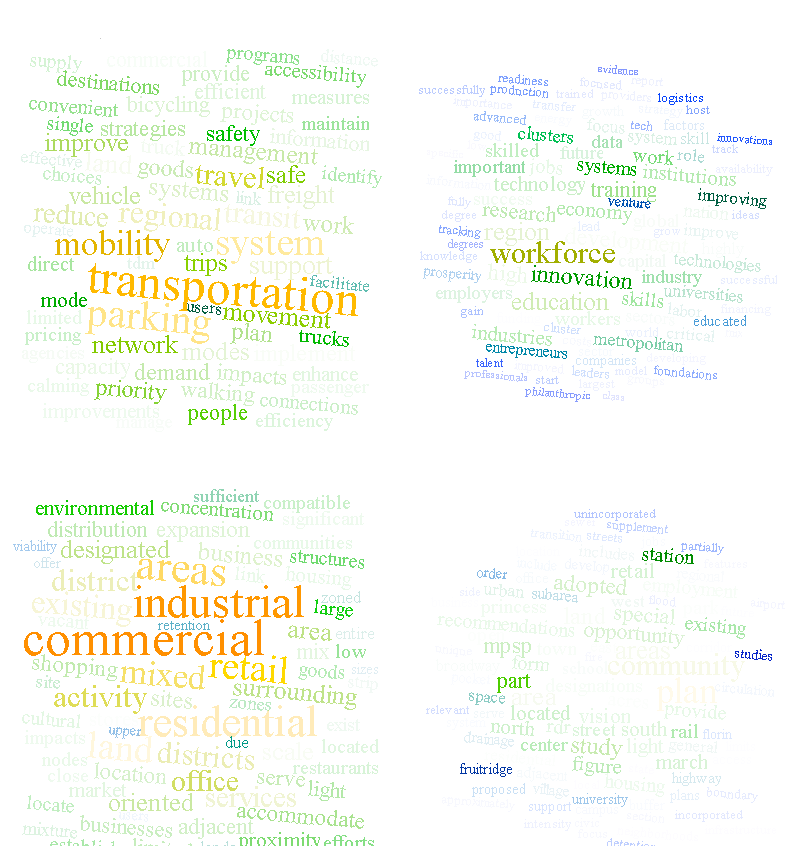
\includegraphics[scale=0.3]{figs/topic_visual}
\end{center}
\end{plain}

%-------------------------------------------------%
\section[Topic Modelling]{Topic Modelling}

\begin{plain}{Model of Topics}
\begin{columns}
\column{0.3\textwidth}
\begin{center}
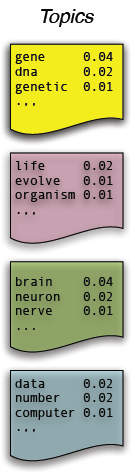
\includegraphics[scale=0.4]{figs/blei_topics}
\end{center}
\column{0.7\textwidth}
\begin{center}
Topics are distributions over words
\end{center}
\end{columns}
\end{plain}

\begin{plain}{Model of Documents}
\begin{columns}
\column{0.3\textwidth}
\begin{center}
Documents have distribution of topics
\end{center}
\column{0.7\textwidth}
\begin{center}
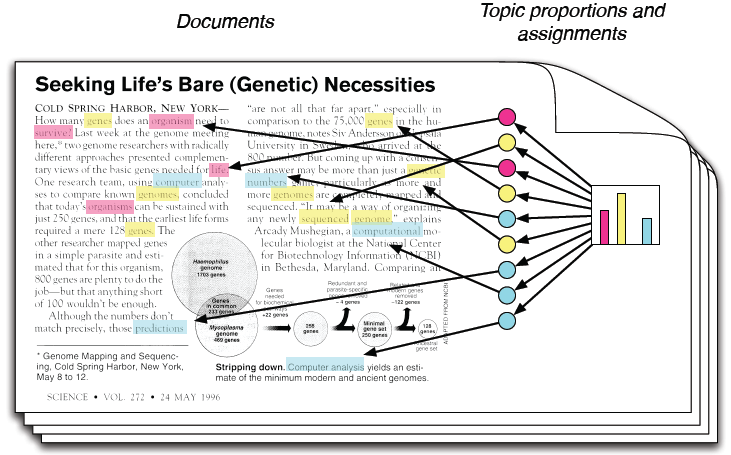
\includegraphics[scale=0.3]{figs/blei_docs}
\end{center}
\end{columns}
\end{plain}

\begin{plain}{Topic Modelling}
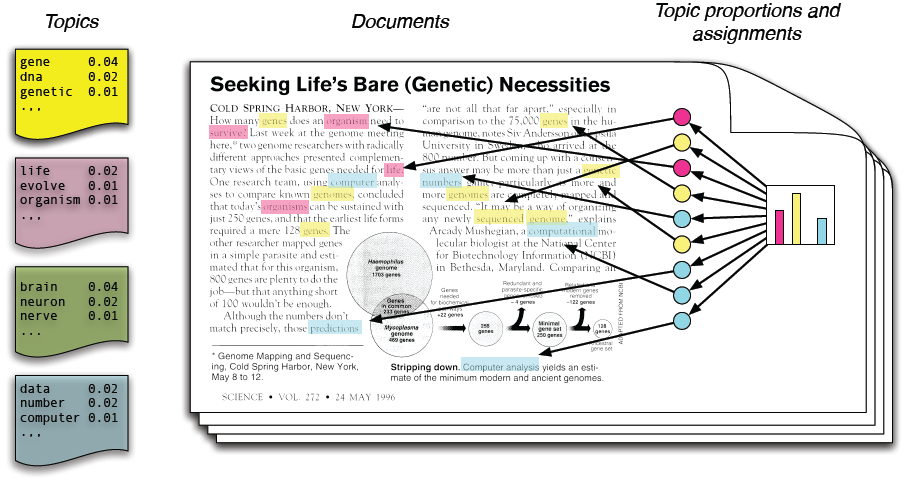
\includegraphics[scale=0.35]{figs/blei}
\end{plain}

\begin{plain}{Word-topic Matrix}
\begin{center}
\vspace{-2ex}
Extracted: Word-topic matrix
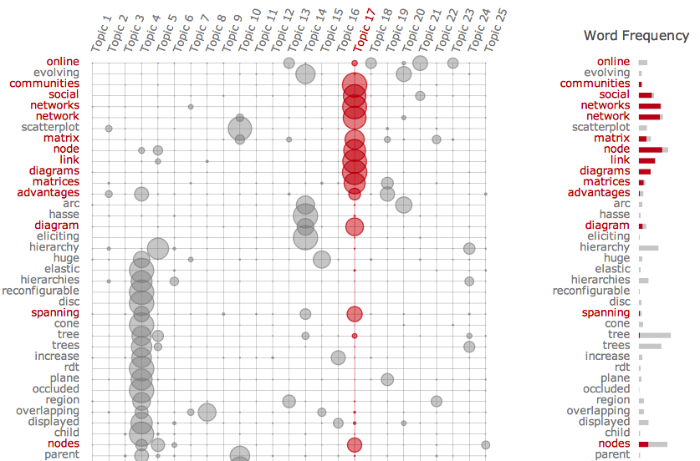
\includegraphics[scale=0.36]{figs/word_topic}\\
Aim: Find document-topic matrix
\end{center}
\end{plain}

\begin{plain}{Steps}
\begin{itemize}
	\p Assume documents are generated by probabilistic model with unknown variables\\
	\p Infer hidden structure onto document\\
	\p Situate new document into model\\
\end{itemize}
TODO: Redo pic
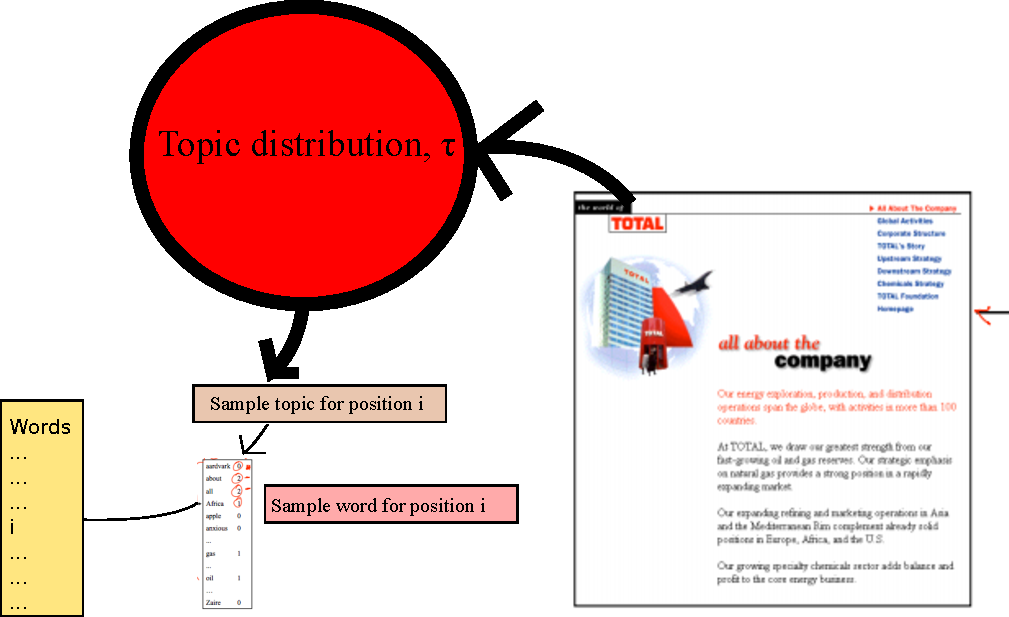
\includegraphics[scale=0.4]{figs/steps}
\end{plain}

\begin{plain}{Approximate Inference \& Provable Guarantees}
\begin{itemize}
	\p Document-topic inference is NP-hard.
	\p Approximate techniques used
	\p Need provably polynomial-time algorithms
\end{itemize}
TODO: Draw pic
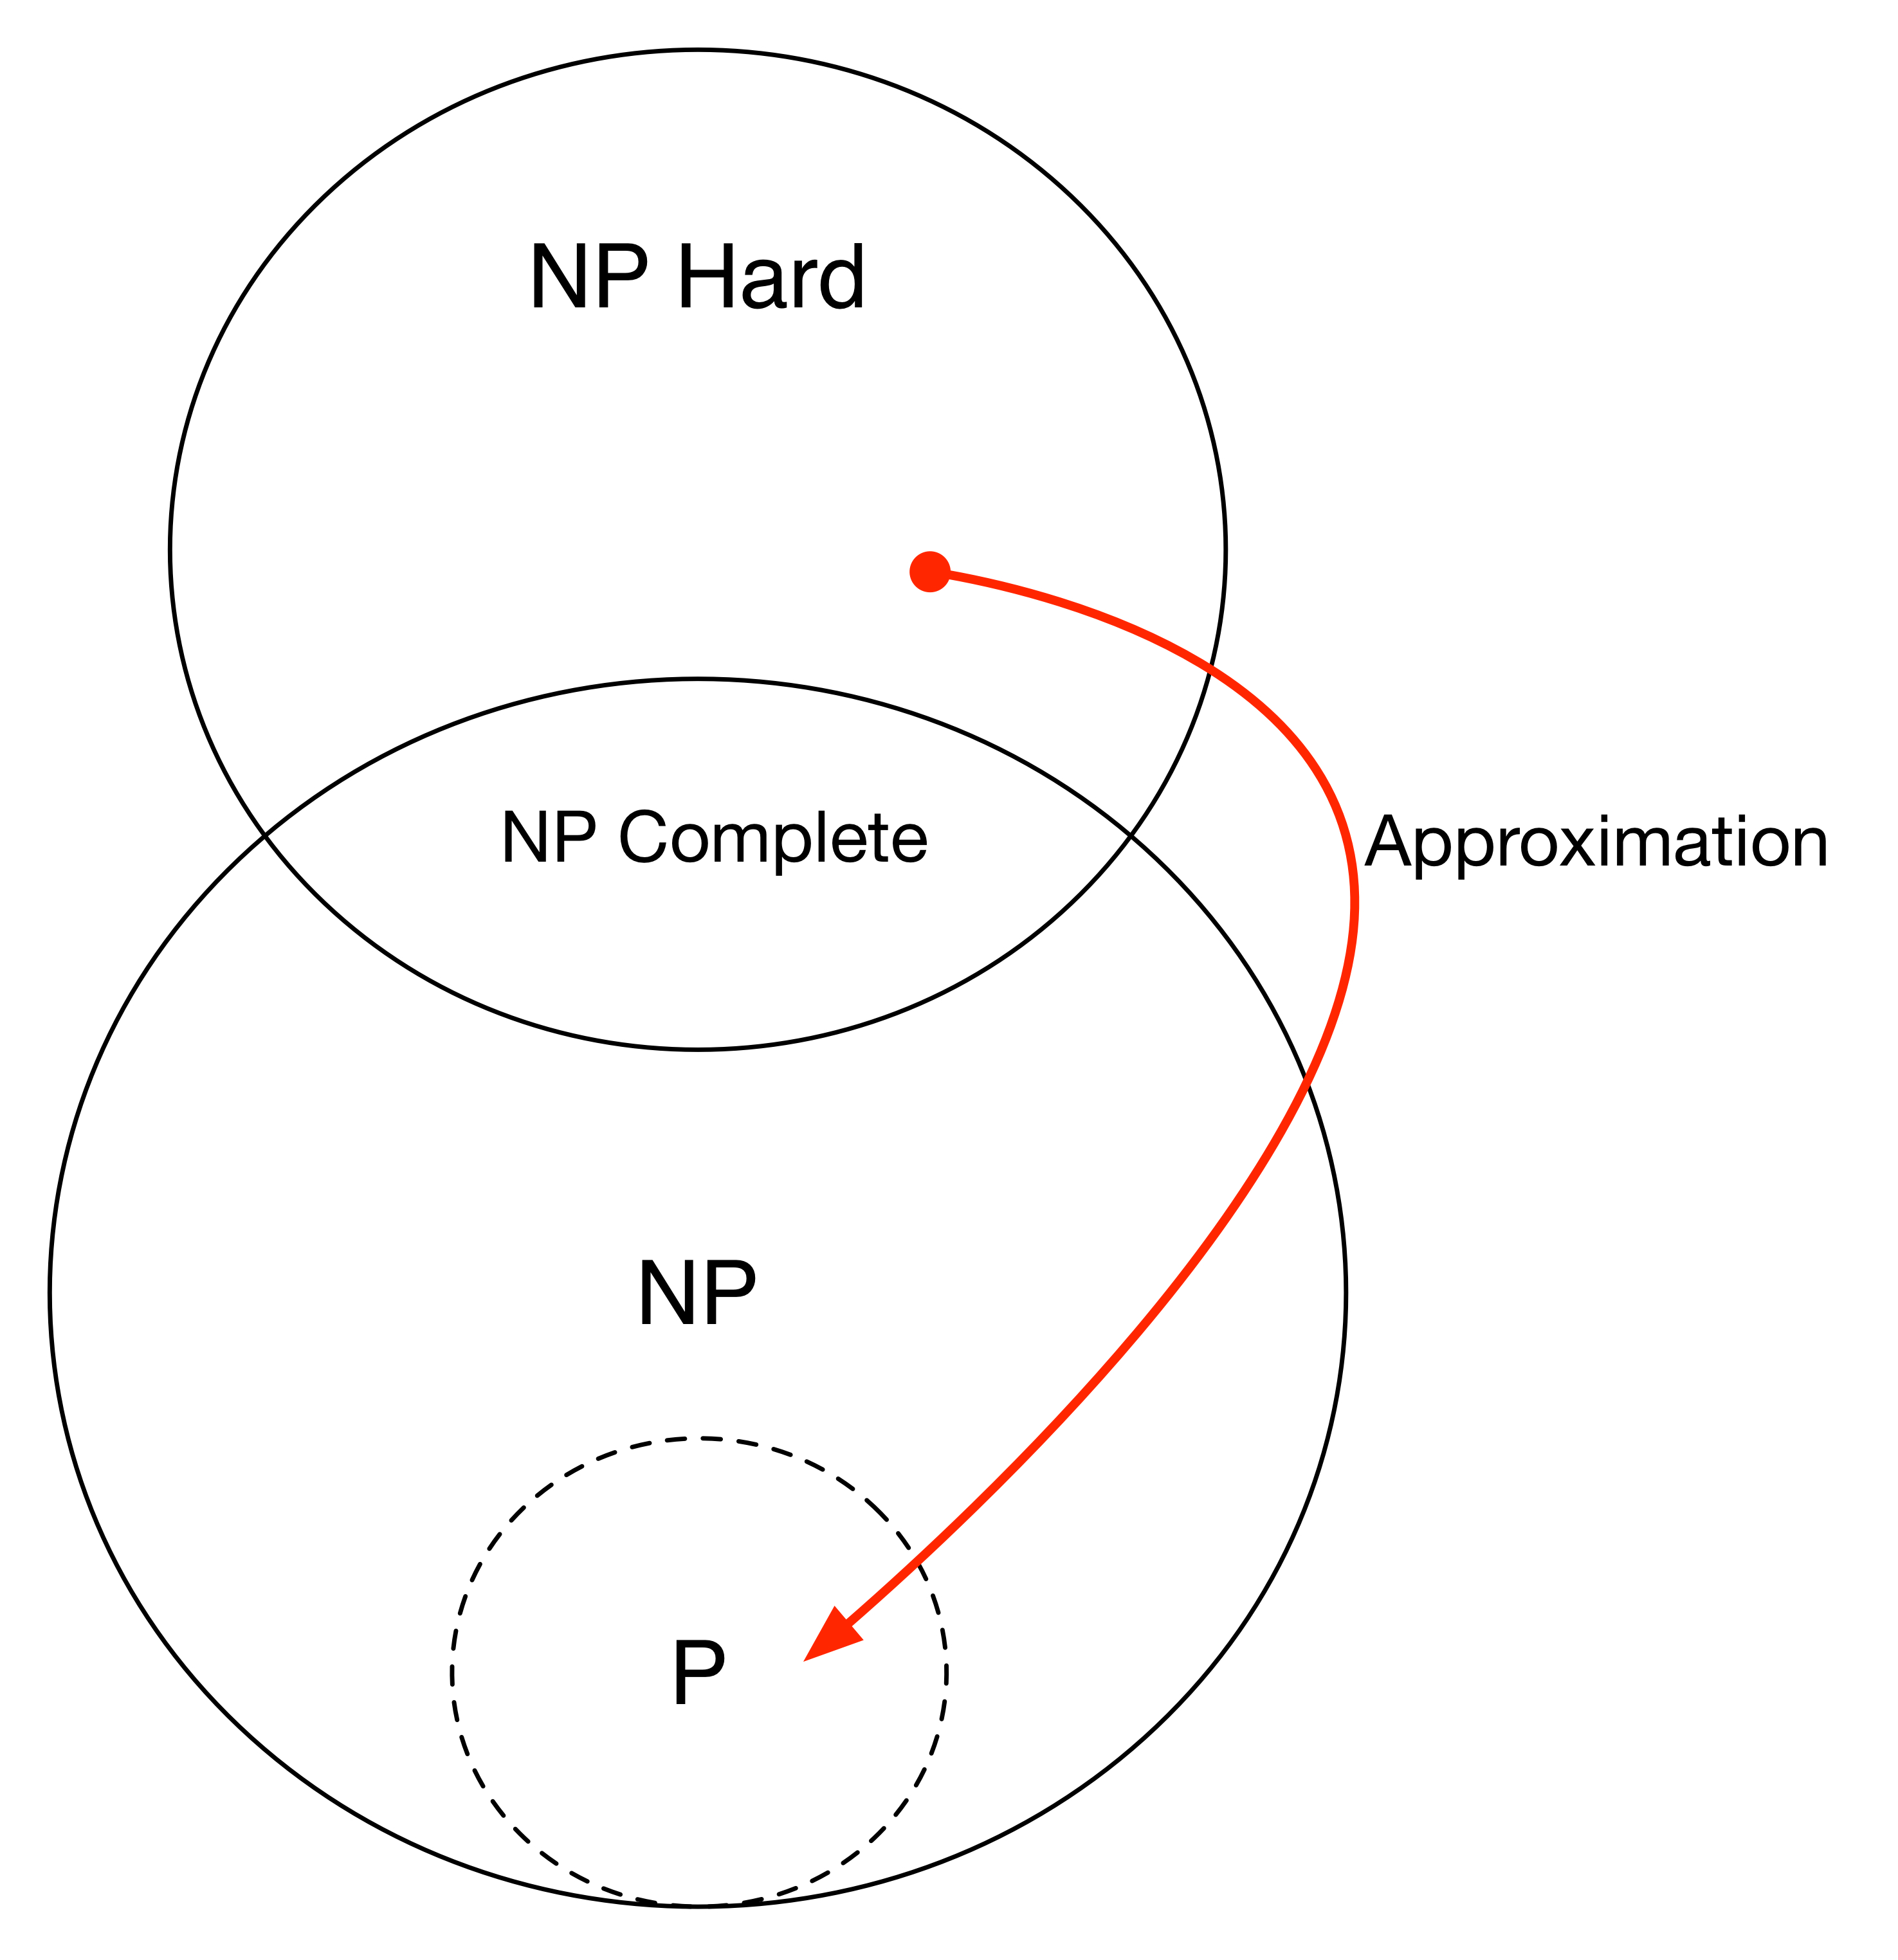
\includegraphics{figs/np_approx}
\end{plain}

%-------------------------------------------------%
\section[Algorithm]{Algorithm}

\begin{plain}{Algorithm}
Steps
\begin{enumerate}
	\p Second order moment matrix of word-word co-occurrences
	\p Anchor word selection
	\p Topic distribution recovery
\end{enumerate}

Assumptions:
	\begin{itemize}
		\p Topics may be correlated
		\p Word-topic distributions are separable
	\end{itemize}
\end{plain}

\begin{plain}{Anchor Words}
\end{plain}

\begin{plain}{LDA}
\end{plain}



\begin{plain}{Contributions}
\end{plain}

%-------------------------------------------------%
\section[Topic Recovery]{Topic Recovery via Bayes' Rule}

%-------------------------------------------------%
\section[Anchor Words]{Efficiently Finding Anchor Words}

%-------------------------------------------------%
\section[Results]{Experimental Results}

%-------------------------------------------------%
\section[Conclusion]{Conclusion}


\end{document}
